\documentclass[a4paper,11pt]{report}
\usepackage{chuan_math_gkt}
\usetikzlibrary{angles,quotes,intersections,patterns,decorations.pathreplacing}
\chuanexamsetup

\begin{document}
\examfontsize

\examsecret{绝密$\bigstar$启用前}

\examtitle{2024年普通高等学校招生全国统一考试（新课标II卷）}{数\quad 学}

\noticetitle
\begin{examnotice}
\item 答卷前，考生务必将自己的姓名、准考证号填写在答题卡上. 
\item 回答选择题时，选出每小题的答案后，用铅笔把答题卡上对应题目的答案标号涂黑. 如需改动，用橡皮擦干净后，再选涂其他答案标号. 回答非选择题时，将答案写在答题卡上. 写在本试卷上无效. 
\item 考试结束后，将本试卷和答题卡一并交回. 
\end{examnotice}

\examsection{一、单项选择题：本大题共8小题，每小题5分，共40分. 在每小题给出的四个选项中，只有一个选项是正确的. 请把正确的选项填涂在答题卡相应的位置上. }
\begin{examquestions}
\item 已知 $z=-1-\mathrm{i}$，则 $|z|=$
\fourchoices{$0$}{$1$}{$\sqrt2$}{$2$}
\item 已知命题 $p:\forall x\in\mathbb R, |x+1|>1$；命题 $q:\exists x>0,x^3=x$，则
\twochoices{$p$ 和 $q$ 都是真命题}{$\neg p$ 和 $q$ 都是真命题}{$p$ 和 $\neg q$ 都是真命题}{$\neg p$ 和 $\neg q$ 都是真命题}
\item 已知向量 $\vec a,\vec b$ 满足 $|\vec a|=1,|\vec a+2\vec b|=2$，且 $(\vec b-2\vec a)\perp\vec b$，则 $|\vec b|=$
\fourchoices{\tallchoice{$\dfrac12$}}{\tallchoice{$\dfrac{\sqrt2}{2}$}}{\tallchoice{$\dfrac{\sqrt3}{2}$}}{$1$}
\item 某农业研究部门在面积相等的100块稻田上种植一种新型水稻，得到各块稻田的亩产量（单位：kg）并部分整理下表：
\begin{tightcenter}
\begin{tabular}{|c|c|c|c|c|c|}
\hline 亩产量 & $[900,950)$ & $[950,1000)$ & $[1000,1050)$ & $[1100,1150)$ & $[1150,1200)$\\ \hline
频数 & 6 & 12 & 18 & 24 & 10\\ \hline
\end{tabular}
\end{tightcenter}
据表中数据，结论中正确的是
\onechoices{100块稻田亩产量的中位数小于1050kg}{100块稻田中亩产量低于1100kg的稻田所占比例超过80\%}{100块稻田亩产量的极差介于200kg至300kg之间}{100块稻田亩产量的平均值介于900kg至1000kg之间}
\item 已知曲线 $C:x^2+y^2=16(y>0)$，从 $C$ 上任意一点 $P$ 向 $x$ 轴作垂线段 $PP'$，$P'$ 为垂足，则线段 $PP'$ 的中点 $M$ 的轨迹方程为
\twochoices{\tallchoice{$\dfrac{x^2}{16}+\dfrac{y^2}{4}=1(y>0)$}}{\tallchoice{$\dfrac{x^2}{16}+\dfrac{y^2}{8}=1(y>0)$}}{\tallchoice{$\dfrac{y^2}{16}+\dfrac{x^2}{4}=1(y>0)$}}{\tallchoice{$\dfrac{y^2}{16}+\dfrac{x^2}{8}=1(y>0)$}}
\item 设函数 $f(x)=a(x+1)^2-1$，$g(x)=\cos x+2ax$，当 $x\in(-1,1)$ 时，曲线 $y=f(x)$ 与 $y=g(x)$ 恰有一个交点，则 $a=$
\fourchoices{$-1$}{\tallchoice{$\dfrac12$}}{$1$}{$2$}
\item 已知正三棱台 $ABC-A_1B_1C_1$ 的体积为 $\dfrac{52}{3}$，$AB=6$，$A_1B_1=2$，则 $A_1A$ 与平面 $ABC$ 所成角的正切值为
\fourchoices{\tallchoice{$\dfrac12$}}{$1$}{$2$}{$3$}
\item 设函数 $f(x)=(x+a)\ln(x+b)$，若 $f(x)\geq0$，则 $a^2+b^2$ 最小值为
\fourchoices{\tallchoice{$\dfrac18$}}{\tallchoice{$\dfrac14$}}{\tallchoice{$\dfrac12$}}{$1$}
\end{examquestions}
\examsection{二、多项选择题：本大题共3小题，每小题6分，共18分. 在每小题给出的四个选项中，有多项符合题目要求. 全部选对得6分，选对但不全得部分分，有选错得0分. }
\begin{examquestions}[start=9]
\item 对于函数 $f(x)=\sin2x$ 和 $g(x)=\sin\left(2x-\dfrac\pi4\right)$，下列正确的有
\twochoices{$f(x)$ 与 $g(x)$ 有相同零点}{$f(x)$ 与 $g(x)$ 有相同最大值}{$f(x)$ 与 $g(x)$ 有相同最小正周期}{$f(x)$ 与 $g(x)$ 的图像有相同的对称轴}
\item 抛物线 $C:y^2=4x$ 的准线为 $l$，$P$ 为 $C$ 上的动点，过 $P$ 作 $\odot A:x^2+(y-4)^2=1$ 的一条切线，$Q$ 为切点，过 $P$ 作 $l$ 的垂线，垂足为 $B$，则
\onechoices{$l$ 与 $\odot A$ 相切}{当 $P,A,B$ 三点共线时，$|PQ|=\sqrt{15}$}{当 $|PB|=2$ 时，$PA\perp AB$}{满足 $|PA|=|PB|$ 的点 $P$ 有且仅有2个}
\item 设函数 $f(x)=2x^3-3ax^2+1$，则
\onechoices{当 $a>1$ 时，$f(x)$ 有三个零点}{当 $a<0$ 时，$x=0$ 是 $f(x)$ 的极大值点}{存在 $a,b$，使得 $x=b$ 为曲线 $y=f(x)$ 的对称轴}{存在 $a$，使得点 $(1,f(1))$ 为曲线 $y=f(x)$ 的对称中心}
\end{examquestions}
\examsection{三、填空题：本大题共3小题，每小题5分，共15分. }
\begin{examquestions}[start=12]
\item 记 $S_n$ 为等差数列 $\{a_n\}$ 的前 $n$ 项和，若 $a_3+a_4=7$，$3a_2+a_5=5$，则 $S_{10}=\blank$. 
\item 已知 $\alpha$ 为第一象限角，$\beta$ 为第三象限角，$\tan\alpha+\tan\beta=4$，$\tan\alpha\tan\beta=\sqrt2+1$，则 $\sin(\alpha+\beta)=\blank$. 
\item 在如图的 $4\times4$ 方格表中选4个方格，要求每行和每列均恰有一个方格被选中，则共有\blank 种选法，在所有符合上述要求的选法中，选中方格中的4个数之和的最大值是\blank. 
\begin{tightcenter}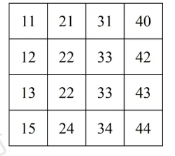
\includegraphics[width=3.4cm]{figures/2024_xgk2_q14.png}\end{tightcenter}
\end{examquestions}
\examsection{四、解答题：本题共5小题，共77分. 解答应写出文字说明、证明过程或演算步骤. }
\begin{examanswers}[start=15]
\item（13分）

记 $\triangle ABC$ 的内角 $A,B,C$ 的对边分别为 $a,b,c$，已知 $\sin A+\sqrt3\cos A=2$. 

（1）求 $A$；

（2）若 $a=2$，$\sqrt2b\sin C=c\sin2B$，求 $\triangle ABC$ 的周长. 
\item（15分）

已知函数 $f(x)=e^x-ax-a^3$. 

（1）当 $a=1$ 时，求曲线 $y=f(x)$ 在点 $(1,f(1))$ 处的切线方程；

（2）若 $f(x)$ 有极小值，且极小值小于0，求 $a$ 的取值范围. 
\item（15分）

如图，平面四边形 $ABCD$ 中，$AB=8$，$CD=3$，$AD=5\sqrt3$，$\angle ADC=90^\circ$，$\angle BAD=30^\circ$，点 $E,F$ 满足 $\dfrac{AE}{ED}=\dfrac25$，$AF=\dfrac12AB$，将 $\triangle AEF$ 沿 $EF$ 对折至 $\triangle PEF$，使得 $PC=4\sqrt3$. 

\noindent\begin{minipage}[t]{0.64\linewidth}
（1）证明：$EF\perp PD$；

（2）求面 $PCD$ 与面 $PBF$ 所成的二面角的正弦值. 
\end{minipage}\hfill
\begin{minipage}[t]{0.30\linewidth}
\vspace{-0.6em}
\centering
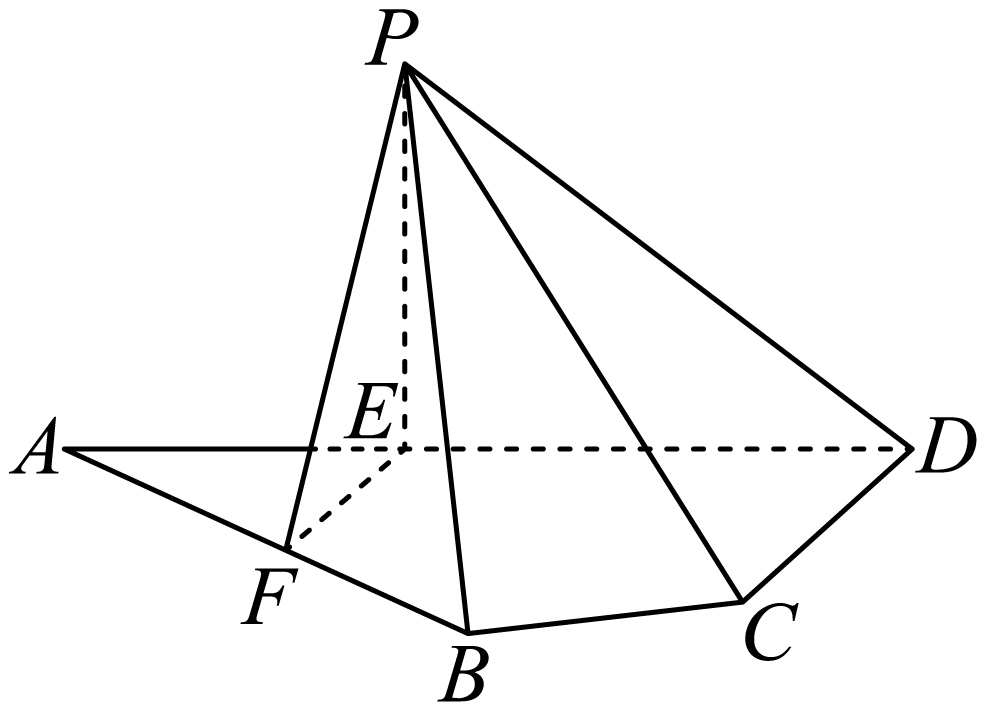
\includegraphics[width=\linewidth]{figures/2024_xgk2_q17.png}
\end{minipage}
\item（17分）

某投篮比赛分为两个阶段，每个参赛队由两名队员组成，比赛具体规则如下：第一阶段由参赛队中一名队员投篮3次，若3次都未投中，则该队被淘汰，比赛成员为0分；若至少投中一次，则该队进入第二阶段，由该队的另一名队员投篮3次，每次投中得5分，未投中得0分. 该队的比赛成绩为第二阶段的得分总和. 某参赛队由甲、乙两名队员组成，设甲每次投中的概率为 $p$，乙每次投中的概率为 $q$，各次投中与否相互独立. 

（1）若 $p=0.4$，$q=0.5$，甲参加第一阶段比赛，求甲、乙所在队比赛成绩不少于5分的概率. 

（2）假设 $0<p<q$，

（i）为使得甲、乙所在队的比赛成绩为15分的概率最大，应该由谁参加第一阶段比赛？

（ii）为使得甲、乙所在队的比赛成绩的数学期望最大，应该由谁参加第一阶段比赛？
\item（17分）

已知双曲线 $C:x^2-y^2=m(m>0)$，点 $P_1(5,4)$ 在 $C$ 上，$k$ 为常数，$0<k<1$. 按照如下方式依次构造点 $P_n(n=2,3,\cdots)$，过 $P_{n-1}$ 作斜率为 $k$ 的直线与 $C$ 的左支交于点 $Q_{n-1}$，令 $P_n$ 为 $Q_{n-1}$ 关于 $y$ 轴的对称点，记 $P_n$ 的坐标为 $(x_n,y_n)$. 

（1）若 $k=\dfrac12$，求 $x_2,y_2$；

（2）证明：数列 $\{x_n-y_n\}$ 是公比为 $\dfrac{1+k}{1-k}$ 的等比数列；

（3）设 $S_n$ 为 $\triangle P_nP_{n+1}P_{n+2}$ 的面积，证明：对任意的正整数 $n$，$S_n=S_{n+1}$. 
\end{examanswers}

\end{document}
